% 15-minute talk, three speakers. Organised by the proposal: the three research questions, what we expected, what we added while testing, and the conclusions.
% One idea per frame, one page per frame; the concept is built up in the order of the slides (no overlay steps).  Build: pdflatex slides.tex (twice).  Speaker notes are kept outside git (slides_notes.tex).
\documentclass[aspectratio=169,11pt]{beamer}
\usetheme{Madrid}
\usecolortheme{default}
\setbeamertemplate{navigation symbols}{}
\usepackage[table]{xcolor}
\usepackage{booktabs,array,tabularx,tikz,pgfplots}
\usetikzlibrary{arrows.meta,calc}
\pgfplotsset{compat=1.17}
\newcommand{\ci}[2]{[#1,\,#2]}
\setbeamerfont{frametitle}{size=\large\bfseries}
% small tag on the title bar: who speaks
\newcommand{\spk}[1]{\begin{tikzpicture}[remember picture,overlay]\node[anchor=north east,font=\scriptsize,text=white] at ([xshift=-0.25cm,yshift=-0.14cm]current page.north east) {Speaker #1};\end{tikzpicture}}
\title[How fast does a recommender go stale?]{How Fast Does a News Recommender Go Stale?}
\subtitle{CS4.406 Information Retrieval and Extraction, Term Project}
\author[Jacob, Joji, Kavuri]{Noel Alex Jacob (2025201085) \and Emil Joji (2025201040) \and Kspsvln Siddardha Kumar Kavuri (2025201061)}
\institute{IIIT Hyderabad, Monsoon 2026}
\date{}

% charts, drawn once and shown in stages (the same axes in every stage, so nothing jumps)
\newcommand{\wordaxis}[2]{\begin{tikzpicture}\begin{axis}[width=6.4cm, height=4.6cm, tick label style={font=\scriptsize}, label style={font=\small}, grid=major, grid style={gray!25}, xlabel={lag (days after the fit)}, ylabel={MRR lost ($\times 10^{-3}$)}, xmin=0.5, xmax=13.5, ymin=-0.6, ymax=8, legend style={font=\scriptsize, at={(0.5,1.03)}, anchor=south, legend columns=-1, draw=none}, xtick={1,3,5,7,9,11,13}]
\addplot[red!70!black, thick, mark=*, mark size=0.8pt, error bars/.cd, y dir=both, y explicit] coordinates {(1,0.0000) +- (0,0.0000) (2,1.2490) +- (0,0.2970) (3,0.7750) +- (0,0.3840) (4,0.7320) +- (0,0.4420) (5,0.7010) +- (0,0.4500) (6,1.8230) +- (0,0.5030) (7,3.0060) +- (0,0.6040) (8,3.8750) +- (0,0.5970) (9,5.7750) +- (0,0.6630) (10,6.7370) +- (0,0.7690) (11,4.5880) +- (0,0.8450) (12,3.5400) +- (0,0.9380) (13,5.8710) +- (0,1.1850)};
#1
\legend{#2}
\end{axis}\end{tikzpicture}}
\newcommand{\wordlive}{\addplot[green!45!black, thick, mark=square*, mark size=0.8pt, error bars/.cd, y dir=both, y explicit] coordinates {(1,0.0000) +- (0,0.0000) (2,0.0620) +- (0,0.0310) (3,0.0690) +- (0,0.0370) (4,0.0760) +- (0,0.0420) (5,0.0710) +- (0,0.0440) (6,0.0820) +- (0,0.0520) (7,0.1300) +- (0,0.0620) (8,0.1410) +- (0,0.0710) (9,0.2460) +- (0,0.0880) (10,0.2900) +- (0,0.1060) (11,0.2900) +- (0,0.1300) (12,0.1390) +- (0,0.1240) (13,0.2230) +- (0,0.1830)};}
\newcommand{\trendaxis}[2]{\begin{tikzpicture}\begin{axis}[width=6.4cm, height=4.6cm, tick label style={font=\scriptsize}, label style={font=\small}, grid=major, grid style={gray!25}, xlabel={minutes between the count and the click}, ylabel={MRR}, symbolic x coords={0,5,15,30,60,180,360}, xtick=data, ymin=0, ymax=0.37, legend style={font=\scriptsize, at={(0.97,0.97)}, anchor=north east, draw=none, fill=white, fill opacity=0.8}]
\addplot[blue!70!black, thick, mark=*, mark size=1pt] coordinates {(0,0.3396) (5,0.3179) (15,0.2790) (30,0.2308) (60,0.1632) (180,0.0699) (360,0.0371)};
#1
\legend{#2}
\end{axis}\end{tikzpicture}}
\newcommand{\trendnewest}{\addplot[red!70!black, dashed, thick] coordinates {(0,0.1905) (5,0.1905) (15,0.1905) (30,0.1905) (60,0.1905) (180,0.1905) (360,0.1905)};}
\newcommand{\trendrandom}{\addplot[gray, dotted, thick] coordinates {(0,0.0172) (5,0.0172) (15,0.0172) (30,0.0172) (60,0.0172) (180,0.0172) (360,0.0172)};}

\begin{document}

%%%%%%%%%%%%%%%%%%%%%%%%%%%%%%% SPEAKER 1: what we proposed, how we measure, what we added %%%%%%%%%%%%%%%%%%%%%%%%%%%%%%%
\begin{frame}\titlepage
\end{frame}

\begin{frame}{What we set out to find}\spk{1}
\Large News goes stale in \textbf{hours}, not months.\normalsize
\medskip

{A recommender trained once and then left alone is \textbf{frozen}. It behaves as if the world had not moved.}
\medskip

{Our proposal asked three questions:}
\begin{enumerate}
\item \textbf{RQ1.} How fast does quality fall, and in what shape?
\item \textbf{RQ2.} Which signal falls first (words, meaning or co-clicks), and why?
\item \textbf{RQ3.} How often must the model be rebuilt?
\end{enumerate}
\medskip

{\textbf{What we expected:} co-click history falls most (a new article has no clicks); meaning matching least; a flat curve would also be a valid answer.}
\end{frame}

\begin{frame}{How we test it}\spk{1}
\centering
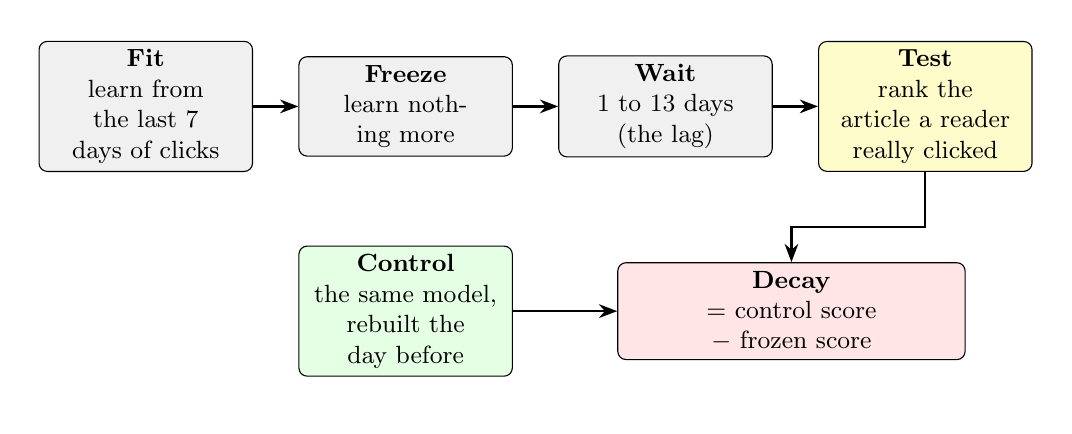
\begin{tikzpicture}[font=\small, box/.style={draw, rounded corners=3pt, align=center, minimum height=1.2cm, text width=2.5cm, inner sep=3pt}, arr/.style={-{Stealth}, thick}]
\path[use as bounding box] (-1.5,-3.8) rectangle (11.4,1.0);
\node[box, fill=gray!12] (a) at (0,0) {\textbf{Fit}\\learn from the last 7 days of clicks};
\node[box, fill=gray!12] (b) at (3.3,0) {\textbf{Freeze}\\learn nothing more};
\node[box, fill=gray!12] (c) at (6.6,0) {\textbf{Wait}\\1 to 13 days\\(the lag)};
\node[box, fill=yellow!20] (d) at (9.9,0) {\textbf{Test}\\rank the article a reader really clicked};
\draw[arr] (a)--(b);
\draw[arr] (b)--(c);
\draw[arr] (c)--(d);
\node[box, fill=green!10] (e) at (3.3,-2.6) {\textbf{Control}\\the same model, rebuilt the day before};
\node[box, fill=red!10, text width=4.2cm] (g) at (8.2,-2.6) {\textbf{Decay}\\= control score $-$ frozen score};
\draw[arr] (e)--(g);
\draw[arr] (d.south)--++(0,-0.7)-|(g.north);
\end{tikzpicture}

\medskip
{Both models are tested on exactly the same clicks. The only difference is the \textbf{age of the model}.}
\end{frame}

\begin{frame}{Scoring one click}\spk{1}
\begin{columns}[T]
\begin{column}{0.47\textwidth}
A reader opens an article. A model ranks the \emph{other} articles. Where does the clicked one land?
\medskip

\small
\begin{tabular}{@{}rlr@{}}
\toprule
Rank & Article (invented list) & Score\\
\midrule
1 & Election results & 0.91\\
2 & Football transfer & 0.74\\
\alert{3} & \alert{\textbf{Storm warning (clicked)}} & \alert{0.66}\\
4 & Cooking recipe & 0.30\\
5 & Celebrity gossip & 0.12\\
\bottomrule
\end{tabular}
\end{column}
\begin{column}{0.50\textwidth}
{\textbf{MRR} (mean reciprocal rank): the score is $1/\text{rank}$, averaged over many clicks. Here: $1/3$.}
\bigskip

{\textbf{AUC}: the chance that the clicked article is ranked above a random other one. 0.5 means random; 1 means perfect.}
\end{column}
\end{columns}
\end{frame}

\begin{frame}{Which other articles do we rank?}\spk{1}
\begin{columns}[T]
\begin{column}{0.48\textwidth}
\textbf{The pool} (main test)

Every article published in the last 48 hours. Many were never shown to this reader.
\medskip

{\small Random order scores MRR 0.0172 \ci{0.0169}{0.0174} ($n=236{,}387$ clicks).}
\end{column}
\begin{column}{0.48\textwidth}
{\textbf{The real slate} (strict test)

Only the articles the site actually showed that reader in that visit: a median of 8 to 9. EB-NeRD only, 25 to 31 May 2023.
\medskip

{\small Random order scores MRR 0.3226 \ci{0.3211}{0.3240} ($n=136{,}674$ clicks).}}
\end{column}
\end{columns}
\bigskip

{Fewer candidates make every score larger. So a pool number is \textbf{never compared} with a slate number.}
\end{frame}

\begin{frame}{What we compare}\spk{1}
\begin{columns}[T]
\begin{column}{0.31\textwidth}
\textbf{Time only}
\begin{itemize}
\item Newest first \emph{(added)}
\end{itemize}
\end{column}
\begin{column}{0.35\textwidth}
{\textbf{The crowd's clicks}
\begin{itemize}
\item Co-click history \emph{(proposed)}
\item Most clicked \emph{(added)}
\item Live trending, the last hour's clicks \emph{(added)}
\end{itemize}}
\end{column}
\begin{column}{0.31\textwidth}
{\textbf{The reader's own reading}
\begin{itemize}
\item Word matching, BM25 \emph{(proposed)}
\item Meaning matching, MiniLM \emph{(proposed)}
\item Genre \emph{(added)}
\end{itemize}}
\end{column}
\end{columns}
\bigskip

{Reference: random order. Main data: EB-NeRD (Danish news). Second sites: NPR and Adressa.}

{Every number has a 95\% interval \ci{low}{high} and the number of clicks, $n$.}
\end{frame}

\begin{frame}{What we added while testing, and why}\spk{1}
\textbf{Better measurement}
\begin{itemize}
\item A control rebuilt the day before: weekdays and weekends differ, so a raw score cannot show decay.
\item An old and a live reader profile: in text models little else is frozen.
\item An hourly axis: the fall happens within hours. Re-reads (15\% of clicks) are dropped.
\end{itemize}
{\textbf{More signals}
\begin{itemize}
\item Genre and live trending: newest first was very strong, and no live click signal had been tried.
\end{itemize}}
{\textbf{Stricter tests}
\begin{itemize}
\item Real slates, the evaluation the proposal intended; two more sites; one-at-a-time checks of our own settings.
\end{itemize}}
\end{frame}

%%%%%%%%%%%%%%%%%%%%%%%%%%%%%%% SPEAKER 2: RQ1 and RQ2 %%%%%%%%%%%%%%%%%%%%%%%%%%%%%%%
\begin{frame}{RQ1. How fast? Click-based signals fall within hours}\spk{2}
\begin{columns}[T]
\begin{column}{0.52\textwidth}
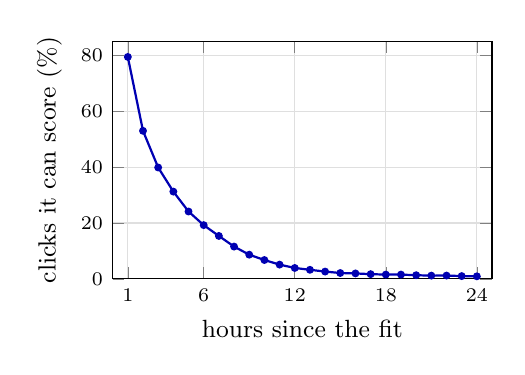
\begin{tikzpicture}
\begin{axis}[width=6.4cm, height=4.6cm, tick label style={font=\scriptsize}, label style={font=\small}, grid=major, grid style={gray!25}, xlabel={hours since the fit}, ylabel={clicks it can score (\%)}, xmin=0, xmax=25, ymin=0, ymax=85, xtick={1,6,12,18,24}]
\addplot[blue!70!black, thick, mark=*, mark size=1pt] coordinates {(1,79.39) (2,52.96) (3,39.85) (4,31.23) (5,24.11) (6,19.24) (7,15.37) (8,11.57) (9,8.67) (10,6.76) (11,5.12) (12,3.92) (13,3.27) (14,2.63) (15,2.11) (16,1.97) (17,1.71) (18,1.55) (19,1.55) (20,1.33) (21,1.18) (22,1.21) (23,1.02) (24,0.93)};
\end{axis}
\end{tikzpicture}
\end{column}
\begin{column}{0.46\textwidth}
\small
Click history, EB-NeRD. The share of clicks it can score:
\medskip

{79.4\% \ci{79.2}{79.6} after 1 hour, 19.2\% \ci{19.1}{19.4} after 6 hours, 0.93\% \ci{0.88}{0.97} after a day.}
\medskip

{It halves every 3.02 h \ci{3.00}{3.03}. In daily terms: 12\% at lag 1, none at lag 7.}
\medskip

{\scriptsize 40 cells per hour, each of up to 5{,}000 clicks.}
\end{column}
\end{columns}
\end{frame}

\begin{frame}{RQ1. How fast? Text signals fall gradually, over days}\spk{2}
\begin{columns}[T]
\begin{column}{0.50\textwidth}
\wordaxis{}{word matching, old profile}
\end{column}
\begin{column}{0.48\textwidth}
\small
Share of the lag-1 score lost, with an old profile (EB-NeRD):
\medskip

\scriptsize
\setlength{\tabcolsep}{3pt}
{\begin{tabular}{@{}lrr@{}}
\toprule
 & lag 7 & lag 13\\
\midrule
Word & 9.7\% \ci{7.8}{11.6} & 18.9\% \ci{15.2}{22.7}\\
Genre & 4.3\% \ci{3.1}{5.4} & 16.9\% \ci{14.6}{19.1}\\
Meaning & 3.0\% \ci{1.4}{4.4} & 5.4\% \ci{1.8}{8.9}\\
\bottomrule
\end{tabular}}
\medskip

\small
{\textbf{Shape:} gradual, close to linear for word and meaning; no cliff; still falling at lag 13. Genre speeds up.}

\scriptsize{$n=135{,}583$ clicks at lag 7, 34{,}479 at lag 13.}
\end{column}
\end{columns}
\end{frame}

\begin{frame}{RQ2. Which signal falls first?}\spk{2}
\begin{enumerate}
\item \textbf{Co-click history and most clicked.} Only 0.93\% \ci{0.88}{0.97} of clicks can still be scored after a day.
\medskip
\item \textbf{Word matching.} Loses 9.7\% \ci{7.8}{11.6} of its score in a week.
\medskip
\item \textbf{Genre.} Loses 4.3\% \ci{3.1}{5.4}.
\medskip
\item \textbf{Meaning matching.} Loses 3.0\% \ci{1.4}{4.4}, and exactly 0 with a live profile.
\end{enumerate}
\bigskip

{As we expected: co-click history first, meaning matching last. Word matching falls faster than meaning matching, but only through the old profile (below).}
\end{frame}

\begin{frame}{RQ2. Why? New articles take over, so co-clicks go blind}\spk{2}
Six hours after the freeze, what share of the next clicks go to articles the model has \textbf{never seen}?
\medskip

\centering
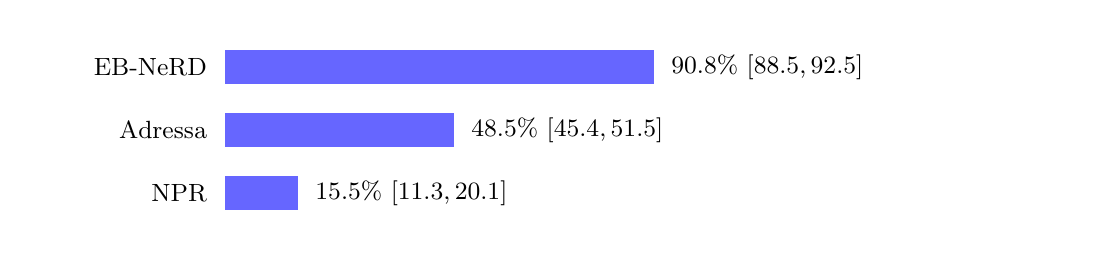
\begin{tikzpicture}[font=\small]
\path[use as bounding box] (-2.4,-2.1) rectangle (11.0,0.5);
\node[anchor=east] at (0,0) {EB-NeRD};
\fill[blue!60] (0.1,-0.22) rectangle (5.55,0.22);
\node[anchor=west] at (5.65,0) {90.8\% \ci{88.5}{92.5}};
\node[anchor=east] at (0,-0.8) {Adressa};
\fill[blue!60] (0.1,-1.02) rectangle (3.01,-0.58);
\node[anchor=west] at (3.11,-0.8) {48.5\% \ci{45.4}{51.5}};
\node[anchor=east] at (0,-1.6) {NPR};
\fill[blue!60] (0.1,-1.82) rectangle (1.03,-1.38);
\node[anchor=west] at (1.13,-1.6) {15.5\% \ci{11.3}{20.1}};
\end{tikzpicture}

\raggedright\small
{$n=$ 3.46 M, 1.26 M and 72{,}136 clicks. Half of the next clicks go to unseen articles after 1.76 h \ci{1.63}{1.91}, 6.23 h \ci{5.79}{6.68} and 12.12 h \ci{10.46}{13.80}.}
\medskip

{\normalsize From the article's side: its click rate halves \textbf{1.74 h} \ci{1.72}{1.77} after the peak (3{,}021 articles, 70.6 M clicks).}
\end{frame}

\begin{frame}{RQ2. Why co-click history falls first: cold start}\spk{2}
\begin{itemize}
\item A new article has no clicks yet, so co-click history \textbf{cannot score it}. This was the cold-start diagnostic we proposed: the share of clicks it cannot score is 88.0\% \ci{87.8}{88.1} at lag 1, 99.6\% \ci{99.58}{99.63} at lag 2 and 100\% from lag 3. The loss is one of coverage.
\medskip
\item While it still works, it shows \textbf{older} news: the median age of its top 10 is 33.3 h \ci{33.3}{33.3}, against 23.8 h \ci{23.7}{23.8} for a random list; 81.5\% of its top 10 are over a day old (random 42.4\%), $n=236{,}387$.
\medskip
\item With newest first as a back-up it is \textbf{worse} than newest first alone: 0.0373 \ci{0.0370}{0.0376} against 0.1905 \ci{0.1896}{0.1914}, because the click part pushes older articles up.
\end{itemize}
\end{frame}

\begin{frame}{RQ2. Why text signals fall: the reader's profile ages}\spk{2}
\begin{columns}[T]
\begin{column}{0.50\textwidth}
{\wordaxis{\wordlive}{old profile (frozen), live profile}}
\end{column}
\begin{column}{0.48\textwidth}
\footnotesize
Word matching on EB-NeRD. \textbf{Old profile} = what the reader had read by the fit date. \textbf{Live profile} = their last 50 clicks.
\medskip

\small
{\textbf{Old profile:} 0.0030 \ci{0.0024}{0.0036} lost in a week ($n=135{,}583$).}
\medskip

{\textbf{Live profile:} 0.00013 \ci{0.00007}{0.00019}.}
\medskip

{The clicked article looks less like the old profile as the lag grows: the similarity gap falls by 0.0205 \ci{0.0167}{0.0245} ($n=116{,}893$); with a live profile, by 0.0022 \ci{0.0020}{0.0024} ($n=135{,}233$).}
\medskip

{\textbf{Text goes stale because the reader's recent interests are missing, not because the articles are old.}}
\end{column}
\end{columns}
\end{frame}

\begin{frame}{RQ2. Did the vocabulary or the embedding space go stale?}\spk{2}
\begin{columns}[T]
\begin{column}{0.48\textwidth}
\textbf{Vocabulary} (word matching)
\small
\medskip

Words of the clicked article that no earlier article contained: the extra from staleness is 0.0033 \ci{0.0032}{0.0034} by lag 7 (2.18\% \ci{2.15}{2.20} against 1.85\% \ci{1.83}{1.87} with a fresh vocabulary). It appears at once (0.0028 \ci{0.0027}{0.0029} at lag 2) and hardly grows, while the loss keeps growing.
\medskip

With a live profile the loss is 0.00013 \ci{0.00007}{0.00019}: about 4\% of the old-profile loss.
\end{column}
\begin{column}{0.48\textwidth}
\textbf{Embedding drift} (meaning matching)
\small
\medskip

The clicked article moves away from the centroid of the last week's articles: 0.0079 \ci{0.0078}{0.0080} by lag 7 and 0.0109 \ci{0.0107}{0.0111} by lag 13.
\medskip

But meaning matching with a live profile loses exactly 0: the drift alone costs nothing.
\end{column}
\end{columns}
\bigskip

\footnotesize $n=135{,}583$ clicks at lag 7, 34{,}479 at lag 13. Across lags the diagnostics and the loss rise together (Spearman 0.50 \ci{0.44}{0.62} for word, 0.79 \ci{0.50}{0.85} for meaning) but both depend on the lag; within a lag the evidence is mixed. Both mechanisms are real and small.
\end{frame}

%%%%%%%%%%%%%%%%%%%%%%%%%%%%%%% SPEAKER 3: settings and site, tests added while testing, RQ3, conclusions %%%%%%%%%%%%%%%%%%%%%%%%%%%%%%%
\begin{frame}{Do our settings or the site decide the size?}\spk{3}
\begin{columns}[T]
\begin{column}{0.48\textwidth}
\textbf{Our settings: hardly.}
\small
\medskip

{One change at a time: pool of 24 or 72 hours; fit window of 10 days; profile of 10 to 200 clicks; word-matching settings; another group of readers; another seed; four times the clicks.}
\medskip

{Word matching loses between 0.0020 \ci{0.0013}{0.0027} and 0.0045 \ci{0.0038}{0.0053} by lag 7 (main run 0.0030 \ci{0.0024}{0.0036}, $n=135{,}583$).}
\end{column}
\begin{column}{0.48\textwidth}
{\textbf{The site: yes.}
\small
\medskip

Word matching, old profile, lost by lag 7:
\begin{itemize}
\item EB-NeRD: 9.7\% \ci{7.8}{11.6}
\item NPR: 0.0043 \ci{0.0040}{0.0046} of 0.0230 (19\%, $n=198{,}746$)
\item Adressa: 0.0144 \ci{0.0139}{0.0148} of 0.0505 (29\%, $n=426{,}503$)
\end{itemize}}
\smallskip

{\footnotesize The percentages for NPR and Adressa are our arithmetic. Turnover orders the click-based time scale (hours on EB-NeRD), not these text losses. Adressa is indicative only.}
\end{column}
\end{columns}
\end{frame}

\begin{frame}{Added test. Live trending: the strongest signal, the fastest to age}\spk{3}
\begin{columns}[T]
\begin{column}{0.52\textwidth}
{\trendaxis{\trendnewest\trendrandom}{trending (1 h count), newest first, random}}
\end{column}
\begin{column}{0.46\textwidth}
\small
Count the clicks an article got from \emph{all} readers in the last hour. Nothing is fitted, so nothing is frozen.
\medskip

{It scores 0.3396 \ci{0.3383}{0.3410}, against 0.1905 \ci{0.1896}{0.1914} for newest first ($n=236{,}387$). It also leads on NPR and Adressa.}
\medskip

{But it ages in minutes: a third of its score is gone after 30 minutes, and it is at 0.0699 \ci{0.0692}{0.0707} after 3 hours.}
\end{column}
\end{columns}
\end{frame}

\begin{frame}{Added test. Real slates: ``newest first'' is no better than random}\spk{3}
\scriptsize EB-NeRD, the articles the site actually showed, $n=136{,}674$ clicks, 25 to 31 May 2023.
\smallskip

\centering\small
\setlength{\tabcolsep}{5pt}
\begin{tabular}{@{}lrr@{}}
\toprule
Scorer & MRR & AUC\\
\midrule
Random order & 0.3226 \ci{0.3211}{0.3240} & 0.4991 \ci{0.4973}{0.5008}\\
{Site's own order} & {0.3239 \ci{0.3224}{0.3254}} & {0.5009 \ci{0.4992}{0.5027}}\\
{Newest first} & {0.3176 \ci{0.3162}{0.3192}} & {0.5026 \ci{0.5010}{0.5042}}\\
{Co-click history} & {0.2637 \ci{0.2624}{0.2649}} & {0.4180 \ci{0.4163}{0.4197}}\\
{Meaning matching} & {0.3532 \ci{0.3516}{0.3548}} & {0.5419 \ci{0.5401}{0.5436}}\\
{Genre} & {0.3647 \ci{0.3632}{0.3663}} & {0.5608 \ci{0.5590}{0.5623}}\\
\bottomrule
\end{tabular}

\raggedright\medskip
{\textbullet\ Every article on a slate is fresh, so being new tells nothing. The proposal's own evaluation changes the earlier picture.}\\
{\textbullet\ Co-click history is \emph{below} random: the clicked article is usually too new to have clicks.}\\
{\textbullet\ Meaning and genre help a little.}
\end{frame}

\begin{frame}{Added test. Genre helps, but how much of it is about the person?}\spk{3}
\textbf{Genre} = the share of the reader's recent clicks in the article's category.
\bigskip

{\Large\textbf{0.0598} \ci{0.0586}{0.0610}\normalsize\quad Genre with newest first beats newest first alone (pool, $n=236{,}387$).}
\bigskip

{\Large\textbf{0.0119} \ci{0.0109}{0.0130}\normalsize\quad is lost if every reader gets the same category mix. So most of the gain is the mix of categories, not the person.}
\bigskip

{\Large\textbf{0.0333} \ci{0.0320}{0.0346}\normalsize\quad On real slates the personal part is larger: genre beats the same mix for everyone ($n=136{,}674$).}
\end{frame}

\begin{frame}{RQ3. How often to rebuild? Quality against cost}\spk{3}
\small Word matching, EB-NeRD, 14 days replayed ($n=236{,}387$), rebuilt \ldots
\smallskip

\centering\footnotesize
\begin{tabular}{@{}lrrr@{}}
\toprule
 & every day & every week & only once\\
\midrule
Rebuilds, fit time in total & 14, 29.1 s & 2, 4.2 s & 1, 2.1 s\\
{MRR, old profile} & {0.0310 \ci{0.0306}{0.0314}} & {0.0298 \ci{0.0295}{0.0302}} & {0.0274 \ci{0.0270}{0.0277}}\\
{MRR, live profile} & {0.0325 \ci{0.0321}{0.0329}} & {0.0324 \ci{0.0320}{0.0328}} & {0.0324 \ci{0.0320}{0.0327}}\\
\bottomrule
\end{tabular}

\raggedright\small\medskip
{Old profile: a weekly rebuild stays within 3.9\% of a daily one (our arithmetic) at about one-seventh of the fit time.}

{Live profile: rebuilding gains nothing.}
\medskip

{Click history is the costly one: 21.9 s per fit against 2.1 s for word matching, and it must be rebuilt within hours (RQ1), so a daily grid cannot show its real staleness.}
\end{frame}

\begin{frame}{The proposed hybrid: a weighted sum of the signals}\spk{3}
\begin{itemize}
\item The proposal combined word, meaning and co-click signals into one ranking. We used rank fusion, and tuned the weights on one half of the days.
\medskip
\item On the 48-hour pool \textbf{no setting beat newest first}: 0.1868 \ci{0.1854}{0.1883} against 0.1910 \ci{0.1896}{0.1924} on the other half ($n=118{,}610$).
\medskip
\item On real slates, a fusion with genre \textbf{does beat random}: 0.3548 \ci{0.3533}{0.3564} against 0.3226 \ci{0.3211}{0.3240} ($n=136{,}674$).
\end{itemize}
\end{frame}

\begin{frame}{Conclusions against what we proposed (1)}\spk{3}
\small
\begin{itemize}
\item \textbf{RQ1, how fast: supported, on two time scales.} Click-based signals fall in hours; text signals fall gradually (about a tenth of word matching in a week), with no cliff.
\medskip
\item \textbf{RQ2, which first: as we expected.} Co-click history first, meaning matching last, word matching between them.
\medskip
\item \textbf{RQ2, why: tested.} Cold start explains the click-based fall. Unseen words and embedding drift are real but small: with a live profile they cost 0.00013 and nothing. The reader's profile carries the staleness. Correlations with the loss are mixed.
\medskip
\item \textbf{A flat curve was a valid answer:} it is the result for text with a live profile.
\end{itemize}
\end{frame}

\begin{frame}{Conclusions against what we proposed (2)}\spk{3}
\small
\begin{itemize}
\item \textbf{RQ3, how often: it depends on the signal and the site.} Text with a live profile: never needed within 14 days. Old profile: weekly is enough. Click-based: hourly on a fast site, every few days on a slow one.
\medskip
\item \textbf{Newest first:} the strongest simple reference on the pool, but no better than random on real slates.
\medskip
\item \textbf{Live trending} beats it by 0.149 \ci{0.147}{0.151}, and ages in minutes.
\medskip
\item \textbf{Genre and meaning} are modestly better than random on real slates.
\end{itemize}
\end{frame}

\begin{frame}{What to keep in mind}\spk{3}
\begin{itemize}
\item One main site and one month. Real slates exist only for EB-NeRD, and live trending was not tested on them.
\item On slates, decay is measured against a fit made a week earlier, because no day-before model exists there.
\item On Adressa the old-profile score at lag 1 is above the live-profile score (0.0505 against 0.0364), which we cannot explain. Treat its decay size as indicative.
\item Our intervals resample clicks; across days they are wider.
\end{itemize}
\bigskip

{\Large Thank you. Questions?}
\end{frame}
\end{document}
